% Options for packages loaded elsewhere
\PassOptionsToPackage{unicode}{hyperref}
\PassOptionsToPackage{hyphens}{url}
%
\documentclass[
  english,
  man]{apa6}
\usepackage{lmodern}
\usepackage{amssymb,amsmath}
\usepackage{ifxetex,ifluatex}
\ifnum 0\ifxetex 1\fi\ifluatex 1\fi=0 % if pdftex
  \usepackage[T1]{fontenc}
  \usepackage[utf8]{inputenc}
  \usepackage{textcomp} % provide euro and other symbols
\else % if luatex or xetex
  \usepackage{unicode-math}
  \defaultfontfeatures{Scale=MatchLowercase}
  \defaultfontfeatures[\rmfamily]{Ligatures=TeX,Scale=1}
\fi
% Use upquote if available, for straight quotes in verbatim environments
\IfFileExists{upquote.sty}{\usepackage{upquote}}{}
\IfFileExists{microtype.sty}{% use microtype if available
  \usepackage[]{microtype}
  \UseMicrotypeSet[protrusion]{basicmath} % disable protrusion for tt fonts
}{}
\makeatletter
\@ifundefined{KOMAClassName}{% if non-KOMA class
  \IfFileExists{parskip.sty}{%
    \usepackage{parskip}
  }{% else
    \setlength{\parindent}{0pt}
    \setlength{\parskip}{6pt plus 2pt minus 1pt}}
}{% if KOMA class
  \KOMAoptions{parskip=half}}
\makeatother
\usepackage{xcolor}
\IfFileExists{xurl.sty}{\usepackage{xurl}}{} % add URL line breaks if available
\IfFileExists{bookmark.sty}{\usepackage{bookmark}}{\usepackage{hyperref}}
\hypersetup{
  pdftitle={Theoretical Bias, as a function of population parameters},
  pdfauthor={Delacre Marie1},
  pdfkeywords={keywords},
  hidelinks,
  pdfcreator={LaTeX via pandoc}}
\urlstyle{same} % disable monospaced font for URLs
\usepackage{graphicx,grffile}
\makeatletter
\def\maxwidth{\ifdim\Gin@nat@width>\linewidth\linewidth\else\Gin@nat@width\fi}
\def\maxheight{\ifdim\Gin@nat@height>\textheight\textheight\else\Gin@nat@height\fi}
\makeatother
% Scale images if necessary, so that they will not overflow the page
% margins by default, and it is still possible to overwrite the defaults
% using explicit options in \includegraphics[width, height, ...]{}
\setkeys{Gin}{width=\maxwidth,height=\maxheight,keepaspectratio}
% Set default figure placement to htbp
\makeatletter
\def\fps@figure{htbp}
\makeatother
\setlength{\emergencystretch}{3em} % prevent overfull lines
\providecommand{\tightlist}{%
  \setlength{\itemsep}{0pt}\setlength{\parskip}{0pt}}
\setcounter{secnumdepth}{-\maxdimen} % remove section numbering
% Make \paragraph and \subparagraph free-standing
\ifx\paragraph\undefined\else
  \let\oldparagraph\paragraph
  \renewcommand{\paragraph}[1]{\oldparagraph{#1}\mbox{}}
\fi
\ifx\subparagraph\undefined\else
  \let\oldsubparagraph\subparagraph
  \renewcommand{\subparagraph}[1]{\oldsubparagraph{#1}\mbox{}}
\fi
% Manuscript styling
\usepackage{upgreek}
\captionsetup{font=singlespacing,justification=justified}

% Table formatting
\usepackage{longtable}
\usepackage{lscape}
% \usepackage[counterclockwise]{rotating}   % Landscape page setup for large tables
\usepackage{multirow}		% Table styling
\usepackage{tabularx}		% Control Column width
\usepackage[flushleft]{threeparttable}	% Allows for three part tables with a specified notes section
\usepackage{threeparttablex}            % Lets threeparttable work with longtable

% Create new environments so endfloat can handle them
% \newenvironment{ltable}
%   {\begin{landscape}\begin{center}\begin{threeparttable}}
%   {\end{threeparttable}\end{center}\end{landscape}}
\newenvironment{lltable}{\begin{landscape}\begin{center}\begin{ThreePartTable}}{\end{ThreePartTable}\end{center}\end{landscape}}

% Enables adjusting longtable caption width to table width
% Solution found at http://golatex.de/longtable-mit-caption-so-breit-wie-die-tabelle-t15767.html
\makeatletter
\newcommand\LastLTentrywidth{1em}
\newlength\longtablewidth
\setlength{\longtablewidth}{1in}
\newcommand{\getlongtablewidth}{\begingroup \ifcsname LT@\roman{LT@tables}\endcsname \global\longtablewidth=0pt \renewcommand{\LT@entry}[2]{\global\advance\longtablewidth by ##2\relax\gdef\LastLTentrywidth{##2}}\@nameuse{LT@\roman{LT@tables}} \fi \endgroup}

% \setlength{\parindent}{0.5in}
% \setlength{\parskip}{0pt plus 0pt minus 0pt}

% Overwrite redefinition of paragraph and subparagraph by the default LaTeX template
% See https://github.com/crsh/papaja/issues/292
\makeatletter
\renewcommand{\paragraph}{\@startsection{paragraph}{4}{\parindent}%
  {0\baselineskip \@plus 0.2ex \@minus 0.2ex}%
  {-1em}%
  {\normalfont\normalsize\bfseries\itshape\typesectitle}}

\renewcommand{\subparagraph}[1]{\@startsection{subparagraph}{5}{1em}%
  {0\baselineskip \@plus 0.2ex \@minus 0.2ex}%
  {-\z@\relax}%
  {\normalfont\normalsize\itshape\hspace{\parindent}{#1}\textit{\addperi}}{\relax}}
\makeatother

% \usepackage{etoolbox}
\makeatletter
\patchcmd{\HyOrg@maketitle}
  {\section{\normalfont\normalsize\abstractname}}
  {\section*{\normalfont\normalsize\abstractname}}
  {}{\typeout{Failed to patch abstract.}}
\patchcmd{\HyOrg@maketitle}
  {\section{\protect\normalfont{\@title}}}
  {\section*{\protect\normalfont{\@title}}}
  {}{\typeout{Failed to patch title.}}
\makeatother
\shorttitle{Theoretical Bias}
\keywords{keywords\newline\indent Word count: X}
\DeclareDelayedFloatFlavor{ThreePartTable}{table}
\DeclareDelayedFloatFlavor{lltable}{table}
\DeclareDelayedFloatFlavor*{longtable}{table}
\makeatletter
\renewcommand{\efloat@iwrite}[1]{\immediate\expandafter\protected@write\csname efloat@post#1\endcsname{}}
\makeatother
\usepackage{lineno}

\linenumbers
\usepackage{csquotes}
\ifxetex
  % Load polyglossia as late as possible: uses bidi with RTL langages (e.g. Hebrew, Arabic)
  \usepackage{polyglossia}
  \setmainlanguage[]{english}
\else
  \usepackage[shorthands=off,main=english]{babel}
\fi

\title{Theoretical Bias, as a function of population parameters}
\author{Delacre Marie\textsuperscript{1}}
\date{}


\authornote{

Correspondence concerning this article should be addressed to Delacre Marie, . E-mail:

}

\affiliation{\vspace{0.5cm}\textsuperscript{1} ULB}

\begin{document}
\maketitle

\hypertarget{the-bias}{%
\section{The bias}\label{the-bias}}

For all \enquote{biased} estimators, when the population effect size is null so is the bias. We will therefore focus on configurations where there is a non-null population effect size. The sampling distribution of Cohen's \(d_s\) (and therefore its bias) is only known under the assumptions of normality and homoscedasticity. On the other hand, the biases of Glass's \(d_s\), Cohen's \(d^*_s\) and Shieh's \(d_s\) are theoretically known for all configurations where the normality assumption is met. In order to simplify the analysis of their bias, it is convenient to subdivide all configurations into 3 conditions:\\
- when population variances are equal across groups;\\
- when population variances are unequal across groups, with equal sample sizes;\\
- when population variances are unequal across groups, with unequal sample sizes.

\hypertarget{preliminary-note}{%
\subsection{Preliminary note}\label{preliminary-note}}

For all previously mentioned estimators (Cohen's \(d_s\), Glass's \(d_s\), Cohen's \(d^*_s\) and Shieh's \(d_s\)), the theoretical expectency is computed by multiplying the population effect size (respectively \(\delta_{Cohen}\), \(\delta_{Glass}\), \(\delta^*_{Cohen}\) and \(\delta_{Shieh}\)) by the following multiplier coefficient:
\begin{equation} 
\gamma=\frac{\sqrt{\frac{df}{2}} \times \Gamma{\frac{df-1}{2}}}{\Gamma{\frac{df}{2}}}
\label{eq:mc}
\end{equation}
where \(df\) are the degrees of freedom (see the main article). \(\gamma\) is \emph{always} positive, meaning that when the population effect size is not zero, all estimators will overestimate the population effect size. Moreover, its limit tends to 1 when the degrees of freedom (\(df\)) tend to infinity, meaning that the larger the degrees of freedom, the lower the bias.\\
While we focus on the theoretical bias of biased estimators when the normality assumption is met, it is interesting to notice that our main conclusions seem to generalize to :\\
- biased estimators when samples are extracted from symmetric distributions;\\
- unbiased estimators when samples are extracted from heavy-tailed symmetric distributions.

\hypertarget{cohens-bf-d_s-see-table-1}{%
\subsection{\texorpdfstring{Cohen's \(\bf d_s\) (see Table 1)}{Cohen's \textbackslash bf d\_s (see Table 1)}}\label{cohens-bf-d_s-see-table-1}}

Under the assumptions that independant residuals are normally distributed with equal variances, the \textbf{bias} of Cohen's \(d_s\) is a function of total sample size (\(N\)) and the population effect size (\(\delta_{Cohen}\)):

\begin{itemize}
\tightlist
\item
  The larger the population effect size, the more Cohen's \(d_s\) will overestimate \(\delta_{Cohen}\);
\end{itemize}

\begin{figure}
\centering
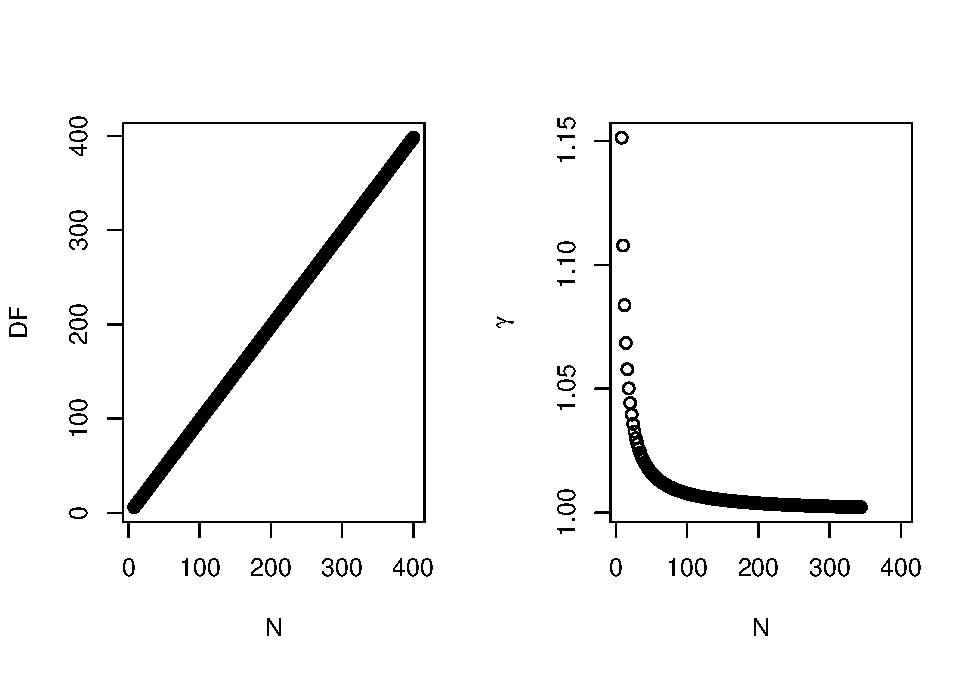
\includegraphics{Theoretical-Bias-of-all-estimators-as-a-function-of-population-parameters_files/figure-latex/biascohendNsize2-1.pdf}
\caption{\label{fig:biascohendNsize2}Degrees of freedom (DF) and \(\gamma\), when computing the bias of Cohen's \(d_s\), when variances are equal across groups, as a function of the total sample size (\(N\)).}
\end{figure}

\begin{itemize}
\item
  The larger the total sample size, the lower the bias (see Figure \ref{fig:biascohendNsize2});
\item
  Of course, considering the degrees of freedom, the sample size ratio does not matter (i.e.~the bias will decrease, whatever one increases \(n_1\), \(n_2\) or both sample sizes).
\end{itemize}

\hypertarget{glasss-bf-d_s-see-table-2}{%
\subsection{\texorpdfstring{Glass's \(\bf d_s\) (see Table 2)}{Glass's \textbackslash bf d\_s (see Table 2)}}\label{glasss-bf-d_s-see-table-2}}

Because degrees of freedom depend only on the control group size (neither on \(\sigma_1\) nor on \(\sigma_2\)), there is no need to distinguish between cases where there is homoscedasticity or heteroscedasticity!

The \textbf{bias} of Glass's \(d_s\) is a function of the control group size (\(n_c\)) and the population effect size (\(\delta_{Glass}\)):

\begin{itemize}
\tightlist
\item
  The larger the population effect size, the more Glass's \(d_s\) will overestimate \(\delta_{Glass}\);
\end{itemize}

\begin{figure}
\centering
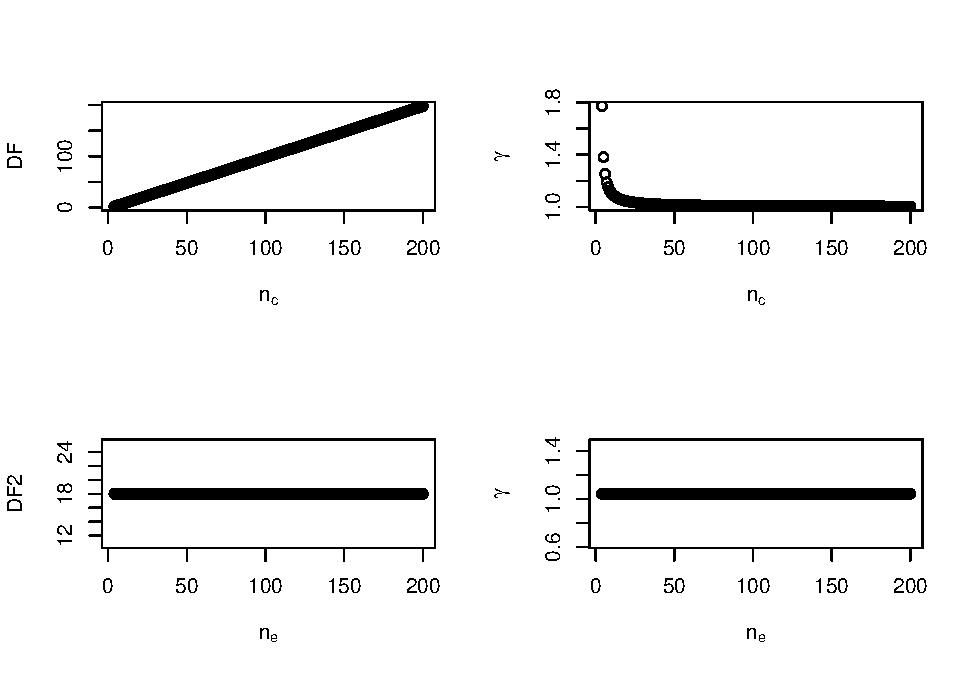
\includegraphics{Theoretical-Bias-of-all-estimators-as-a-function-of-population-parameters_files/figure-latex/biasGlassctrlsize2-1.pdf}
\caption{\label{fig:biasGlassctrlsize2}Degrees of freedom (DF) and \(\gamma\), when computing the bias of Glass's \(d_s\), when variances are equal across groups, as a function of \(n_c\) (top) and \(n_e\) (bottom).}
\end{figure}

\begin{itemize}
\tightlist
\item
  The larger the size of the control group, the lower the bias (see the two top plots in Figure \ref{fig:biasGlassctrlsize2}). On the other hand, increasing the experimental group size does not impact the bias (see the two bottom plots in Figure \ref{fig:biasGlassctrlsize2}).
\end{itemize}

\hypertarget{cohens-bf-d_s-see-table-2}{%
\subsection{\texorpdfstring{Cohen's \(\bf d^*_s\) (see Table 2)}{Cohen's \textbackslash bf d\^{}*\_s (see Table 2)}}\label{cohens-bf-d_s-see-table-2}}

\hypertarget{when-variances-are-equal-across-populations}{%
\subsubsection{When variances are equal across populations}\label{when-variances-are-equal-across-populations}}

When \(\sigma_1=\sigma_2=\sigma\):
\[df_{Cohen's \; d^*_s} = \frac{(n_1-1)(n_2-1)(2\sigma^2)^2}{(n_2-1)\sigma^4+(n_1-1)\sigma^4} = \frac{(n_1-1)(n_2-1)\times 4\sigma^4}{\sigma^4(n_1+n_2-2)} = \frac{4(n_1-1)(n_2-1)}{n_1+n_2-2}\]
One can see that degrees of freedom depend only on the total sample size (\(N\)) and the sample size allocation ratio \(\left( \frac{n_1}{n_2}\right)\). As a consequence, the \textbf{bias} of Cohen's \(d^*_s\) is a function of the population effect size (\(\delta^*_{Cohen}\)), the sample size allocation ratio \(\left( \frac{n_1}{n_2}\right)\) and the total sample size (\(N\)).

\begin{itemize}
\tightlist
\item
  The larger the population effect size, the more Cohen's \(d^*_s\) will overestimate \(\delta^*_{Cohen}\);
\end{itemize}

\begin{figure}
\centering
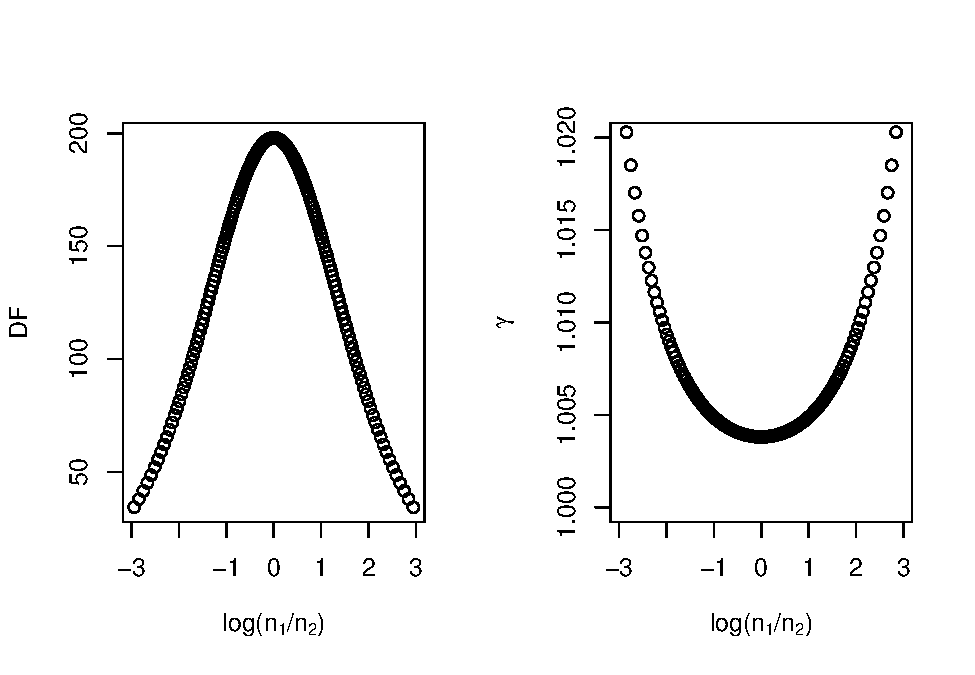
\includegraphics{Theoretical-Bias-of-all-estimators-as-a-function-of-population-parameters_files/figure-latex/biascohendprimehomNratio2-1.pdf}
\caption{\label{fig:biascohendprimehomNratio2}Degrees of freedom (DF) and \(\gamma\), when computing the bias of Cohen's \(d^*_s\), when variances are equal across groups, as a function of the logarithm of the sample sizes ratio \(log\left(\frac{n_1}{n_2} \right)\).}
\end{figure}

\begin{itemize}
\tightlist
\item
  The further the sample size allocation ratio is from 1, the larger the bias (see Figure \ref{fig:biascohendprimehomNratio2});
\end{itemize}

\begin{figure}
\centering
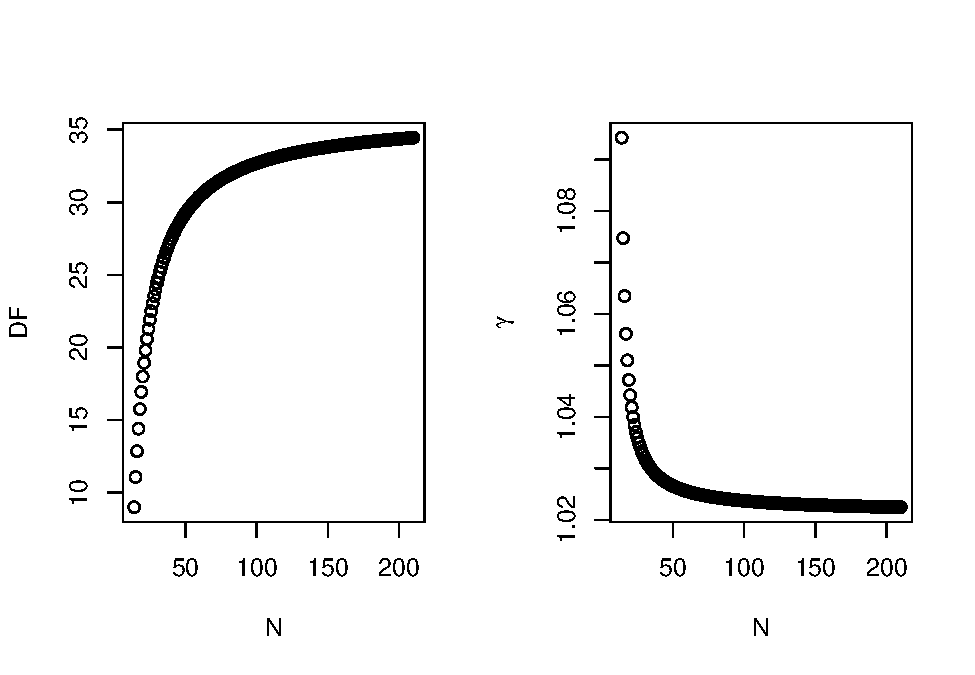
\includegraphics{Theoretical-Bias-of-all-estimators-as-a-function-of-population-parameters_files/figure-latex/biascohendprimehomNsize2-1.pdf}
\caption{\label{fig:biascohendprimehomNsize2}Degrees of freedom (DF) and \(\gamma\), when computing the bias of Cohen's \(d^*_s\), when variances are equal across groups, as a function of the total sample size (\(N\)).}
\end{figure}

\begin{itemize}
\tightlist
\item
  The larger the total sample size, the lower the bias (see Figure \ref{fig:biascohendprimehomNsize2}).
\end{itemize}

\hypertarget{when-variances-are-unequal-across-populations-with-equal-sample-sizes}{%
\subsubsection{When variances are unequal across populations, with equal sample sizes}\label{when-variances-are-unequal-across-populations-with-equal-sample-sizes}}

When \(n_1 = n_2 = n\):
\[df_{Cohen's \; d^*_s} = \frac{(n-1)^2(\sigma^2_1+\sigma^2_2)^2}{(n-1)(\sigma^4_1+\sigma^4_2)} =  \frac{(n-1)(\sigma^4_1+\sigma^4_2+2\sigma^2_1\sigma^2_2)}{\sigma^4_1+\sigma^4_2}\]
One can see that degrees of freedom depend only on the total sample size (\(N\)) and the \(SD\)-ratio \(\left( \frac{\sigma_1}{\sigma_2}\right)\). As a consequence, the \textbf{bias} of Cohen's \(d^*_s\) is a function of the population effect size (\(\delta^*_{Cohen}\)), the \(SD\)-ratio \(\left( \frac{\sigma_1}{\sigma_2}\right)\) and the total sample size (\(N\)):

\begin{itemize}
\tightlist
\item
  The larger the population effect size, the more Cohen's \(d^*_s\) will overestimate \(\delta^*_{Cohen}\);
\end{itemize}

\begin{figure}
\centering
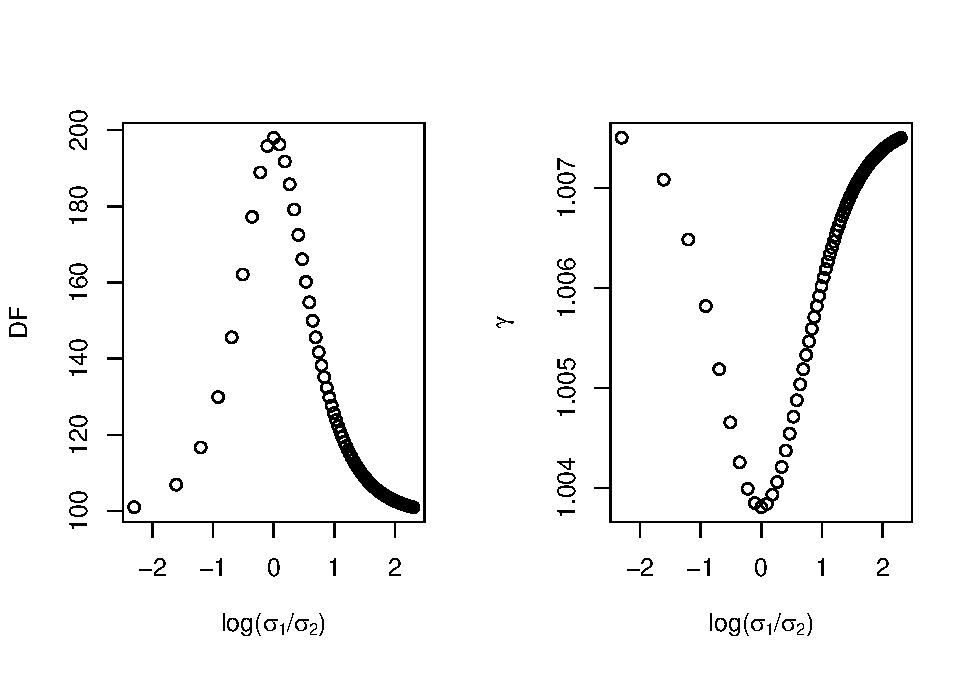
\includegraphics{Theoretical-Bias-of-all-estimators-as-a-function-of-population-parameters_files/figure-latex/biascohendprimehetbalSDratio2-1.pdf}
\caption{\label{fig:biascohendprimehetbalSDratio2}Degrees of freedom (DF) and \(\gamma\), when computing the bias of Cohen's \(d^*_s\), when variances are unequal across groups and sample sizes are equal, as a function of the logarithm of the \(SD\)-ratio (\(log \left( \frac{\sigma_1}{\sigma_2} \right)\)).}
\end{figure}

\begin{itemize}
\tightlist
\item
  The further the \(SD\)-ratio is from 1, the larger the bias (see Figure \ref{fig:biascohendprimehetbalSDratio2});
\end{itemize}

\begin{figure}
\centering
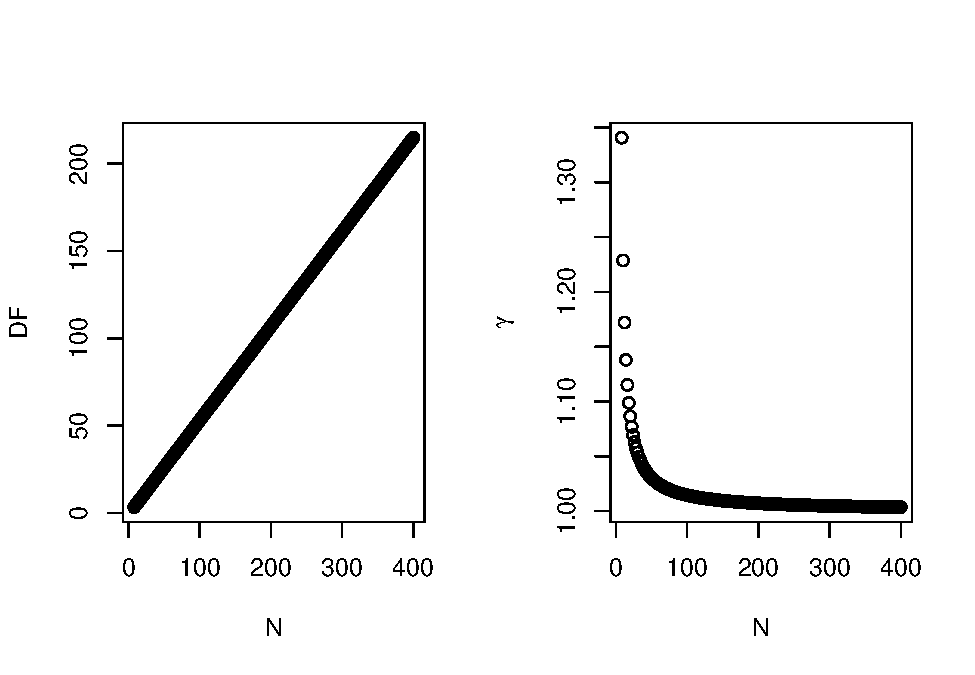
\includegraphics{Theoretical-Bias-of-all-estimators-as-a-function-of-population-parameters_files/figure-latex/biascohendprimehetbalNsize2-1.pdf}
\caption{\label{fig:biascohendprimehetbalNsize2}Degrees of freedom (DF) and \(\gamma\), when computing the bias of Cohen's \(d^*_s\), when variances are unequal across groups and sample sizes are equal, as a function of the total sample size (\(N\)).}
\end{figure}

\begin{itemize}
\tightlist
\item
  The larger the total sample size, the lower the bias (see Figure \ref{fig:biascohendprimehetbalNsize2}).
\end{itemize}

\begin{figure}
\centering
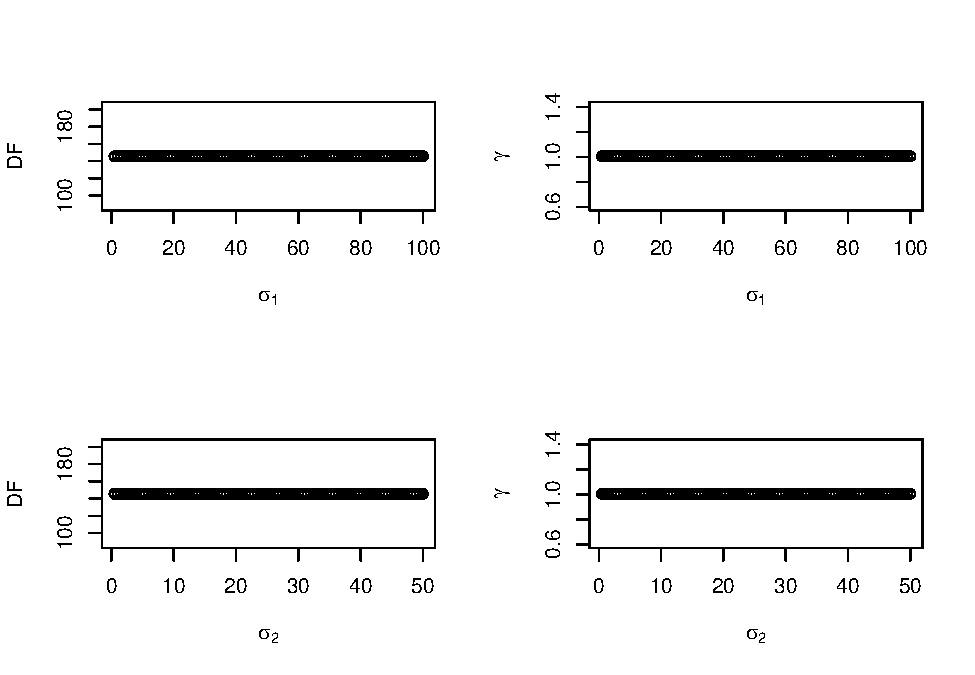
\includegraphics{Theoretical-Bias-of-all-estimators-as-a-function-of-population-parameters_files/figure-latex/biascohendprimehetbalvariance2-1.pdf}
\caption{\label{fig:biascohendprimehetbalvariance2}Degrees of freedom (DF) and \(\gamma\), when computing the bias of Cohen's \(d^*_s\), when variances are unequal across groups and sample sizes are equal, as a function of \(\sigma_1\) (top plots) and \(\sigma_2\) (bottom plots), for a constant \(SD\)-ratio.}
\end{figure}

Note: for a constant \(SD\)-ratio, \(\sigma_1\) and \(\sigma_2\) do not matter (see Figure \ref{fig:biascohendprimehetbalvariance2}).

\hypertarget{when-variances-are-unequal-across-populations-with-unequal-sample-sizes}{%
\subsubsection{When variances are unequal across populations, with unequal sample sizes}\label{when-variances-are-unequal-across-populations-with-unequal-sample-sizes}}

The \textbf{bias} of Cohen's \(d^*_s\) is a function of the population effect size (\(\delta^*_{Cohen}\)), the total sample size (\(N\)), and the interaction between the sample sizes ratio and the \(SD\)-ratio \(\left(\frac{n_1}{n_2}\times\frac{\sigma_1}{\sigma_2} \right)\) :

\begin{itemize}
\tightlist
\item
  The larger the population effect size, the more Cohen's \(d^*_s\) will overestimate \(\delta^*_{Cohen}\);
\end{itemize}

\begin{figure}
\centering
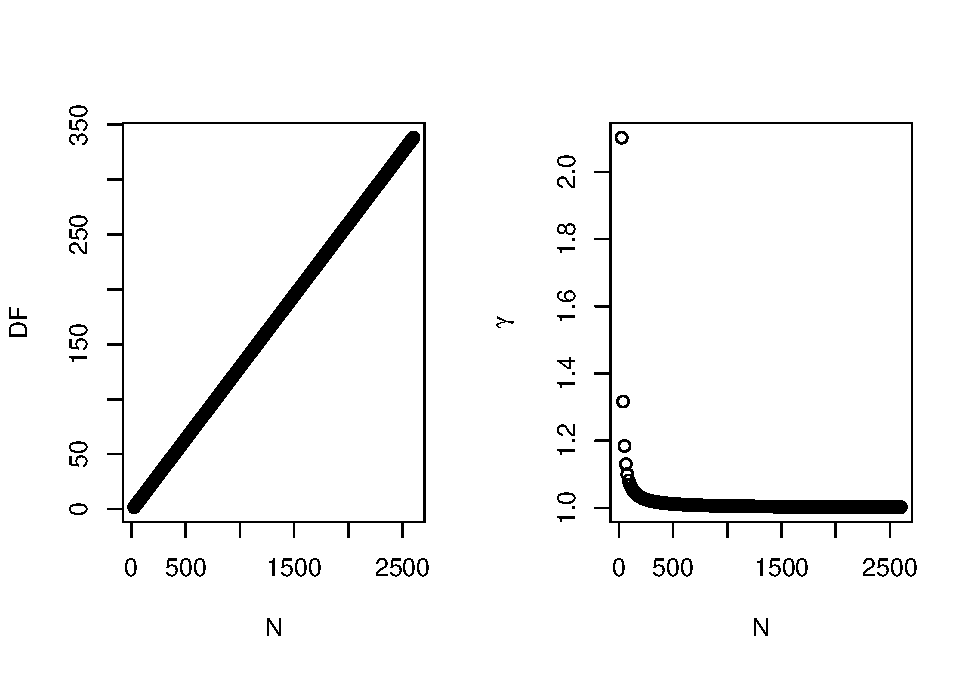
\includegraphics{Theoretical-Bias-of-all-estimators-as-a-function-of-population-parameters_files/figure-latex/biascohendprimehetunbalNsize2-1.pdf}
\caption{\label{fig:biascohendprimehetunbalNsize2}Degrees of freedom (DF) and \(\gamma\), when computing the bias of Cohen's \(d^*_s\), when variances and sample sizes are unequal across groups, as a function of the total sample size (\(N\)).}
\end{figure}

\begin{itemize}
\tightlist
\item
  The larger the total sample size, the lower the bias (see Figure \ref{fig:biascohendprimehetunbalNsize2});
\end{itemize}

\begin{figure}
\centering
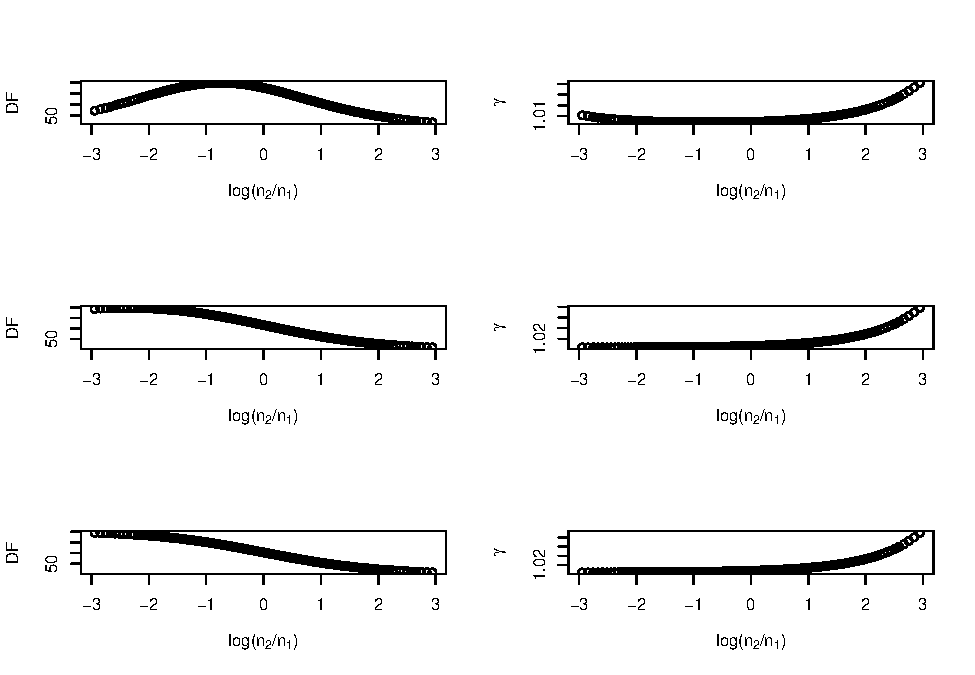
\includegraphics{Theoretical-Bias-of-all-estimators-as-a-function-of-population-parameters_files/figure-latex/biascohendprimehetunbalnratiosdratio2-1.pdf}
\caption{\label{fig:biascohendprimehetunbalnratiosdratio2}Degrees of freedom (\(DF\)) and \(\gamma\), when computing the bias of Cohen's \(d^*_s\) when variances and sample sizes are unequal across groups, as a function of the logarithm of the sample sizes ratio (\(log \left( \frac{n_1}{n_2} \right)\)), when \(SD\)-ratio equals 1.46 (first row), 3.39 (second row) or 7 (third row).}
\end{figure}

\begin{itemize}
\tightlist
\item
  The smallest bias always occurs when there is a positive pairing between variances and sample sizes, because one gives more weight to the smallest variance, in the denominator of the \(df\) computation. Moreover, the further the \(SD\)-ratio is from 1, the further from 1 will also be the sample sizes ratio associated with the smallest bias (see Figure \ref{fig:biascohendprimehetunbalnratiosdratio2}). This can be explained by splitting the numerator and the denominator in the \(df\) computation.
\end{itemize}

\begin{figure}
\centering
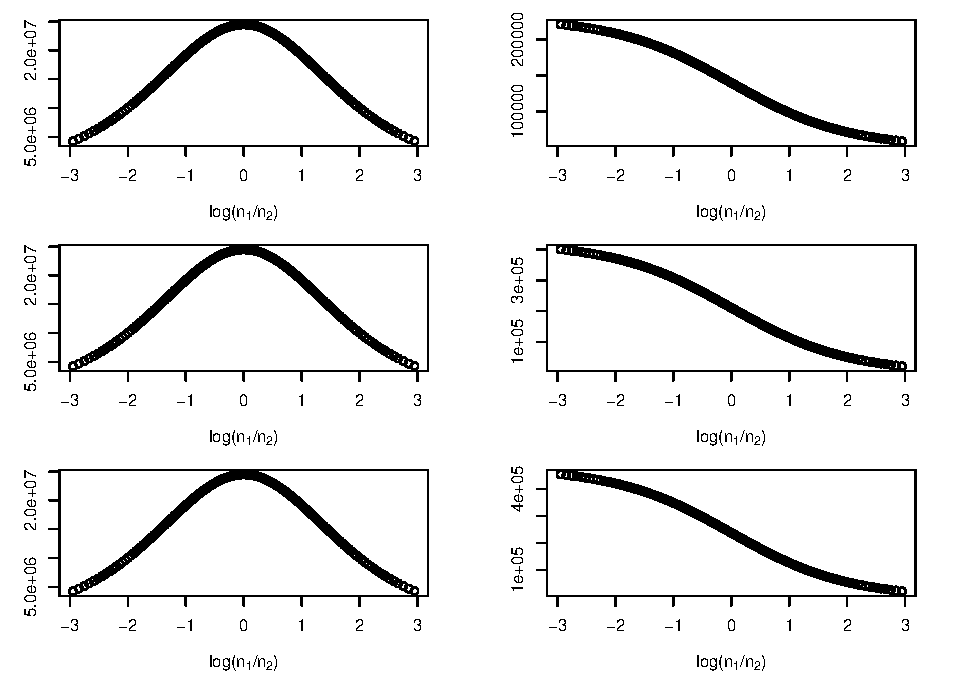
\includegraphics{Theoretical-Bias-of-all-estimators-as-a-function-of-population-parameters_files/figure-latex/dfnumdenomcohendprimehetunbalnratiosdratio2-1.pdf}
\caption{\label{fig:dfnumdenomcohendprimehetunbalnratiosdratio2}Numerator and denominator of the degrees of freedom (\(DF\)) computation, when computing the bias of Cohen's \(d^*_s\) when variances and sample sizes are unequal across groups, as a function of the logarithm of the sample sizes ratio (\(log \left( \frac{n_1}{n_2} \right)\)), when \(SD\)-ratio equals 1.46 (first row), 3.39 (second row) or 7 (third row).}
\end{figure}

As illustrated in Figure \ref{fig:dfnumdenomcohendprimehetunbalnratiosdratio2}, for any \(SD\)-ratio, the numerator of the degrees of freedom will be maximized when sample sizes are equal across groups (and is not impacted by the \(SD\)-ratio). On the other hand, the denominator will be minimized when there is a positive pairing between variances and sample sizes. For example, when \(\sigma_1 > \sigma_2\), the smallest denominator occurs when \(\frac{n_1}{n_2}\) reaches its maximum value and the larger the \(SD\)-ratio, the larger the impact of the sample sizes ratio on the denominator.

\begin{figure}
\centering
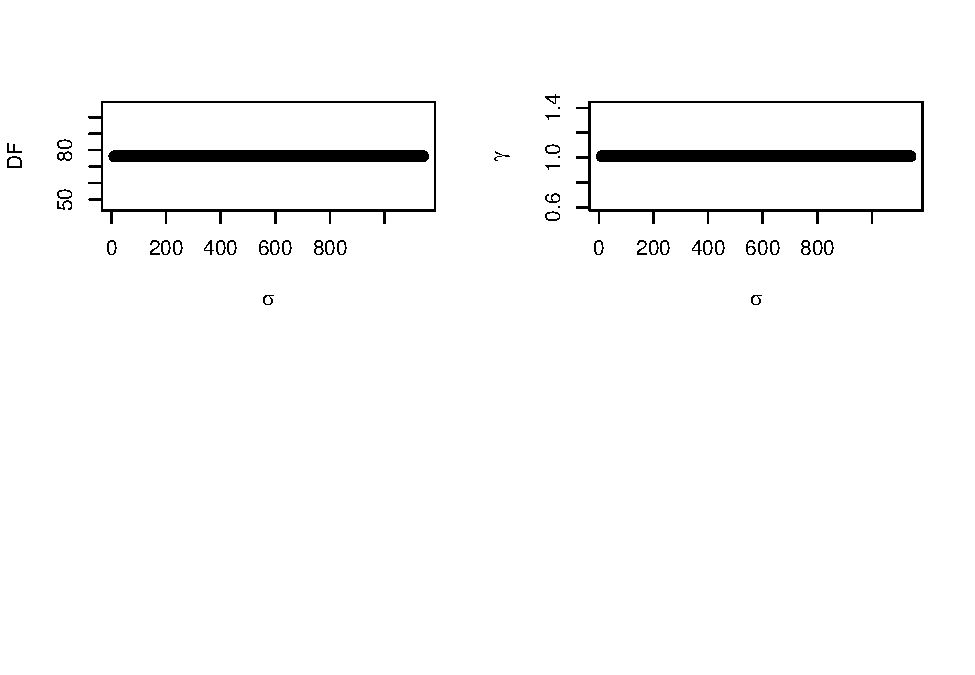
\includegraphics{Theoretical-Bias-of-all-estimators-as-a-function-of-population-parameters_files/figure-latex/biascohendprimehetunbalvariance2-1.pdf}
\caption{\label{fig:biascohendprimehetunbalvariance2}Degrees of freedom (DF) and \(\gamma\), when computing the bias of Cohen's \(d^*_s\), when variances and sample sizes are unequal across groups, as a function of \(\sigma= \frac{(\sigma_1^2+\sigma_2^2)}{2}\), for a constant \(SD\)-ratio.}
\end{figure}

Note: for a constant \(SD\)-ratio, the variance does not matter. (See Figure \ref{fig:biascohendprimehetunbalvariance2}).

\hypertarget{shiehs-bf-d_s-see-table-2}{%
\subsection{\texorpdfstring{Shieh's \(\bf d_s\) (see Table 2)}{Shieh's \textbackslash bf d\_s (see Table 2)}}\label{shiehs-bf-d_s-see-table-2}}

\hypertarget{when-variances-are-equal-across-populations-1}{%
\subsubsection{When variances are equal across populations}\label{when-variances-are-equal-across-populations-1}}

When \(\sigma_1=\sigma_2=\sigma\):
\[df_{Shieh's \; d_s} = \frac{\left( \frac{n_2\sigma^2+n_1\sigma^2}{n_1n_2}\right)^2}{\frac{(n_2-1)\left( \frac{\sigma^2}{n_1}\right)^2+(n_1-1)\left( \frac{\sigma^2}{n_2}\right)^2}{(n_1-1)(n_2-1)}}\]
\[\leftrightarrow df_{Shieh's \; d_s} = \frac{[\sigma^2(n_1+n_2)]^2}{n_1^2n_2^2} \times \frac{(n_1-1)(n_2-1)}{(n_2-1) \times  \frac{\sigma^4}{n_1^2}+(n_1-1) \times \frac{\sigma^4}{n_2^2}}\]
\[\leftrightarrow df_{Shieh's \; d_s} = \frac{\sigma^4N^2}{n_1^2n_2^2} \times \frac{(n_1-1)(n_2-1)}{\sigma^4 \left( \frac{n_2-1}{n^2_1}+\frac{n_1-1}{n^2_2}\right) }\]
\[\leftrightarrow df_{Shieh's \; d_s} = \frac{N^2(n_1-1)(n_2-1)}{n_1^2n_2^2 \left( \frac{n_2^2(n_2-1)+n_1^2(n_1-1)}{n_1^2n_2^2}\right)}\]
\[\leftrightarrow df_{Shieh's \; d_s} = \frac{N^2(n_1-1)(n_2-1)}{n_2^2(n_2-1)+n_1^2(n_1-1)}\]

One can see that degrees of freedom depend only on the total sample size (\(N\)) and the sample size allocation ratio \(\left( \frac{n_1}{n_2}\right)\). As a consequence, the \textbf{bias} of Shieh's \(d^*_s\) is a function of the population effect size (\(\delta_{Shieh}\)), the sample size allocation ratio \(\left( \frac{n_1}{n_2}\right)\) and the total sample size (\(N\)).

\begin{itemize}
\tightlist
\item
  The larger the population effect size, the more Shieh's \(d_s\) will overestimate \(\delta_{Shieh}\);
\end{itemize}

\begin{figure}
\centering
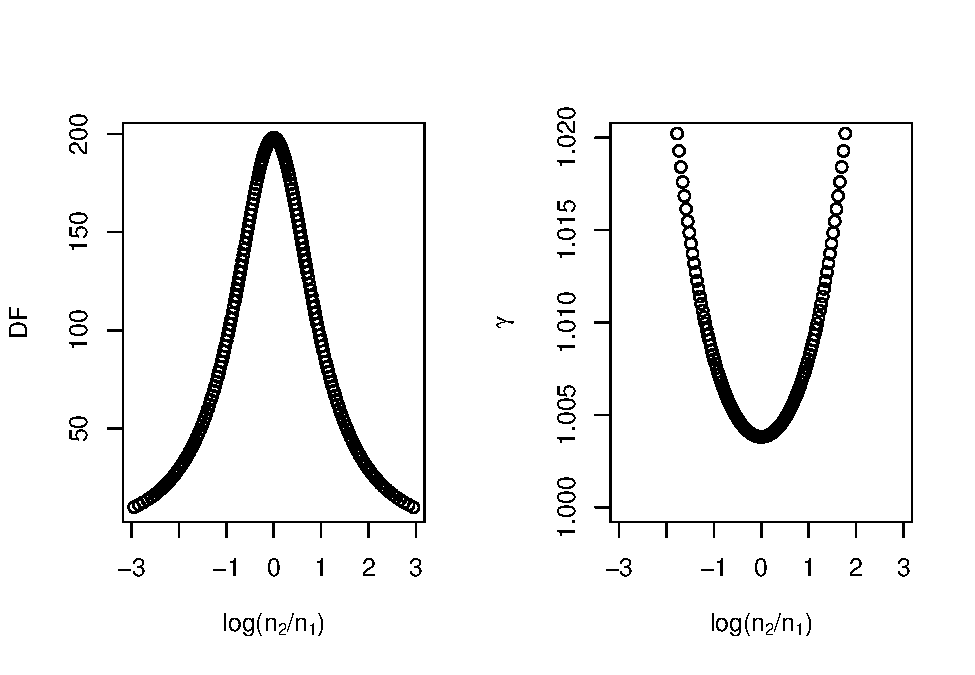
\includegraphics{Theoretical-Bias-of-all-estimators-as-a-function-of-population-parameters_files/figure-latex/biasshiehhomNratio2-1.pdf}
\caption{\label{fig:biasshiehhomNratio2}Degrees of freedom (DF) and \(\gamma\), when computing the bias of Shieh's \(d_s\), when variances are equal across groups, as a function of the logarithm of the sample sizes ratio \((log \left(\frac{n_1}{n_2})\right)\).}
\end{figure}

\begin{itemize}
\tightlist
\item
  The further the sample size allocation ratio is from 1, the larger the bias (see Figure \ref{fig:biasshiehhomNratio2});
\end{itemize}

\begin{figure}
\centering
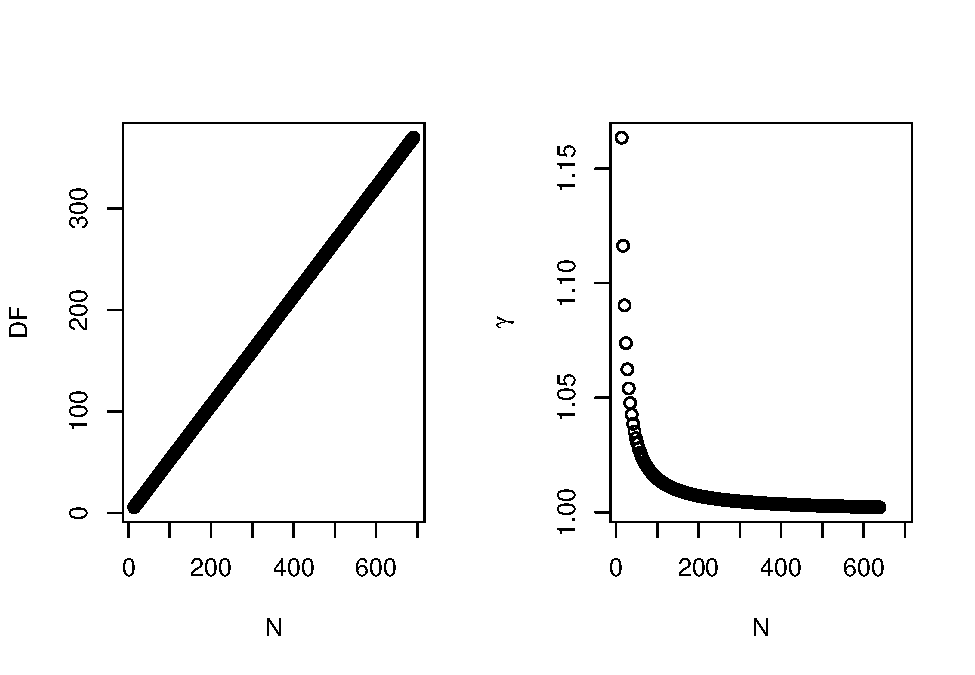
\includegraphics{Theoretical-Bias-of-all-estimators-as-a-function-of-population-parameters_files/figure-latex/biasshiehhomNsize2-1.pdf}
\caption{\label{fig:biasshiehhomNsize2}Degrees of freedom (DF) and \(\gamma\), when computing the bias of Shieh's \(d_s\), when variances are equal across groups, as a function of the total sample size (\(N\)).}
\end{figure}

\begin{itemize}
\tightlist
\item
  For a constant sample sizes ratio, the larger the total sample size, the lower the bias (see Figure \ref{fig:biasshiehhomNsize2}).
\end{itemize}

\begin{figure}
\centering
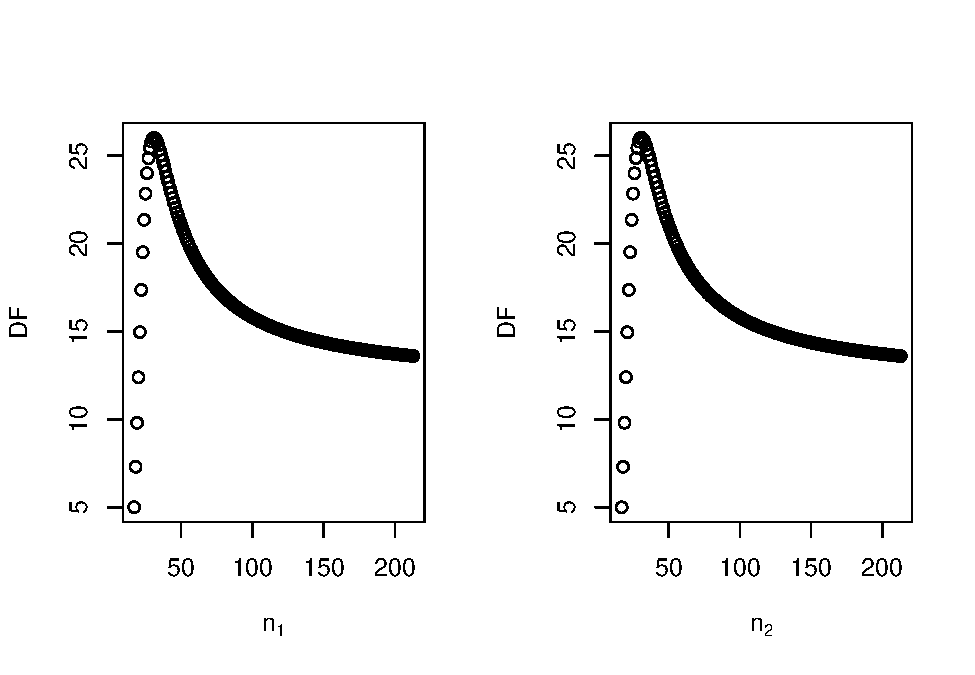
\includegraphics{Theoretical-Bias-of-all-estimators-as-a-function-of-population-parameters_files/figure-latex/biasshiehhomuneqNsize2-1.pdf}
\caption{\label{fig:biasshiehhomuneqNsize2}Degrees of freedom (DF), when computing the bias of Shieh's \(d_s\), when variances are equal across groups, when adding subjects only in the first group (left) or in the second group (right).}
\end{figure}

Note: when computing Cohen's \(d^*_s\), degrees of freedom increased when adding subjects in either one or both groups, even when the sample size ratio increased. When computing Shieh's \(d_s\), this is not true anymore: there is a larger impact of the sample sizes ratio such that increasing the sample sizes ratio when adding subjects in only one group can decrease the degrees of freedom and therefore, increase the bias (See Figure \ref{fig:biasshiehhomuneqNsize2}).

\hypertarget{when-variances-are-unequal-across-populations-with-equal-sample-sizes-1}{%
\subsubsection{When variances are unequal across populations, with equal sample sizes}\label{when-variances-are-unequal-across-populations-with-equal-sample-sizes-1}}

When \(n_1=n_2=n\):
\[df_{Shieh's \; d_s} = \frac{\left( \frac{\sigma_1^2+\sigma_2^2}{n} \right)^2}{\frac{(\sigma_1^2/n)^2+(\sigma_2^2/n)^2}{n-1}}\]
\[\leftrightarrow df_{Shieh's \; d_s} = \frac{(\sigma_1^2+\sigma_2^2)^2}{n^2} \times\frac{n-1}{\frac{\sigma_1^4+\sigma_2^4}{n^2}}\]
\[\leftrightarrow df_{Shieh's \; d_s} = \frac{(\sigma_1^2+\sigma_2^2)^2 \times (n-1)}{\sigma_1^4+\sigma_2^4}\]

One can see that degrees of freedom depend on the total sample size (\(N\)) and the \(SD\)-ratio \(\left( \frac{\sigma_1}{\sigma_2}\right)\). As a consequence, the bias depends on the population effect size (\(\delta_{Shieh}\)), the \(SD\)-ratio \(\left( \frac{\sigma_1}{\sigma_2}\right)\) and the total sample size (\(N\)).

\begin{itemize}
\tightlist
\item
  The larger the population effect size, the more Shieh's \(d_s\) will overestimate \(\delta_{Shieh}\);
\end{itemize}

\begin{figure}
\centering
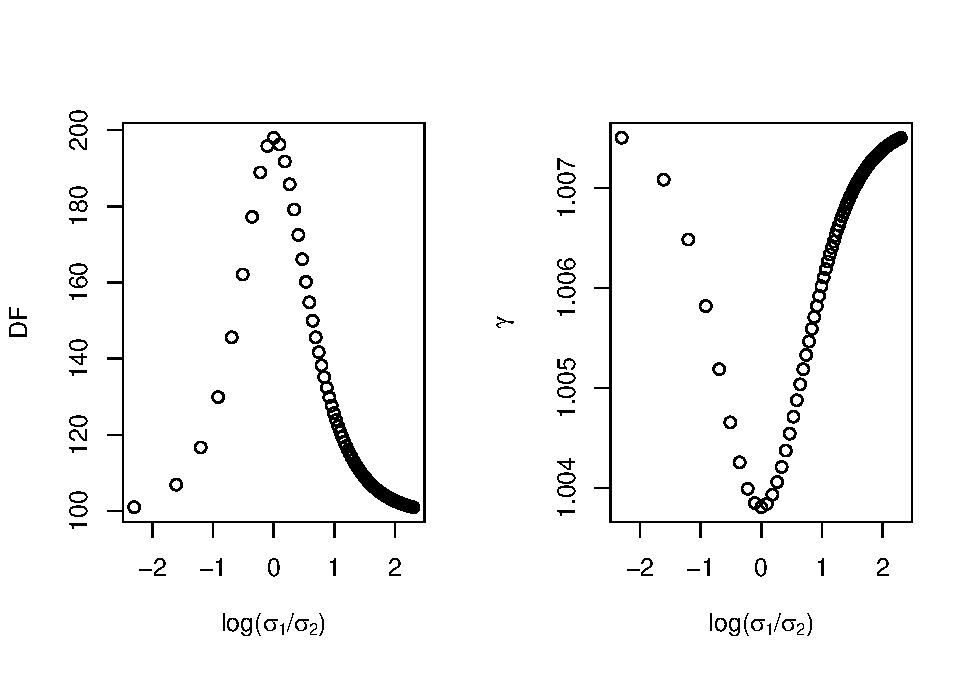
\includegraphics{Theoretical-Bias-of-all-estimators-as-a-function-of-population-parameters_files/figure-latex/biasshiehhetbalSDratio2-1.pdf}
\caption{\label{fig:biasshiehhetbalSDratio2}Degrees of freedom (DF) and \(\gamma\), when computing the bias of Shieh's \(d_s\), when variances are unequal across groups and sample sizes are equal, as a function of the logarithm of the \(SD\)-ratio \((log \left(\frac{\sigma_1}{\sigma_2})\right)\).}
\end{figure}

\begin{itemize}
\tightlist
\item
  The further the \(SD\)-ratio is from 1, the larger the bias (see Figure \ref{fig:biasshiehhetbalSDratio2});
\end{itemize}

\begin{figure}
\centering
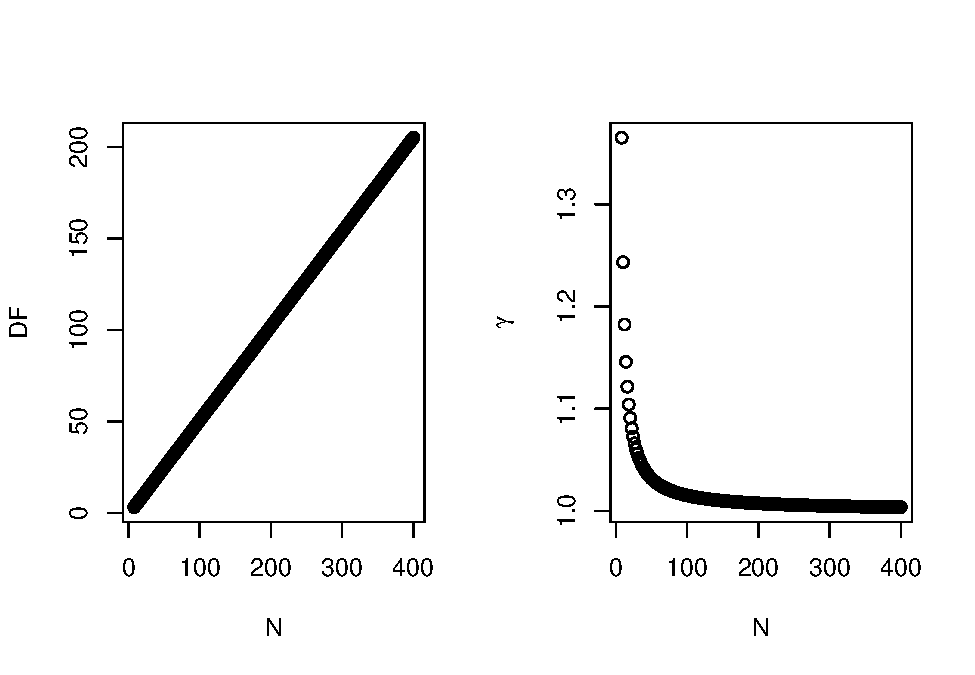
\includegraphics{Theoretical-Bias-of-all-estimators-as-a-function-of-population-parameters_files/figure-latex/biasshiehhetbalNsize2-1.pdf}
\caption{\label{fig:biasshiehhetbalNsize2}Degrees of freedom (DF) and \(\gamma\), when computing the bias of Shieh's \(d_s\), when variances are unequal across groups and sample sizes are equal, as a function of the total sample size (\(N\)).}
\end{figure}

\begin{itemize}
\tightlist
\item
  The larger the total sample size, the lower the bias (see Figure \ref{fig:biasshiehhetbalNsize2});
\end{itemize}

\begin{figure}
\centering
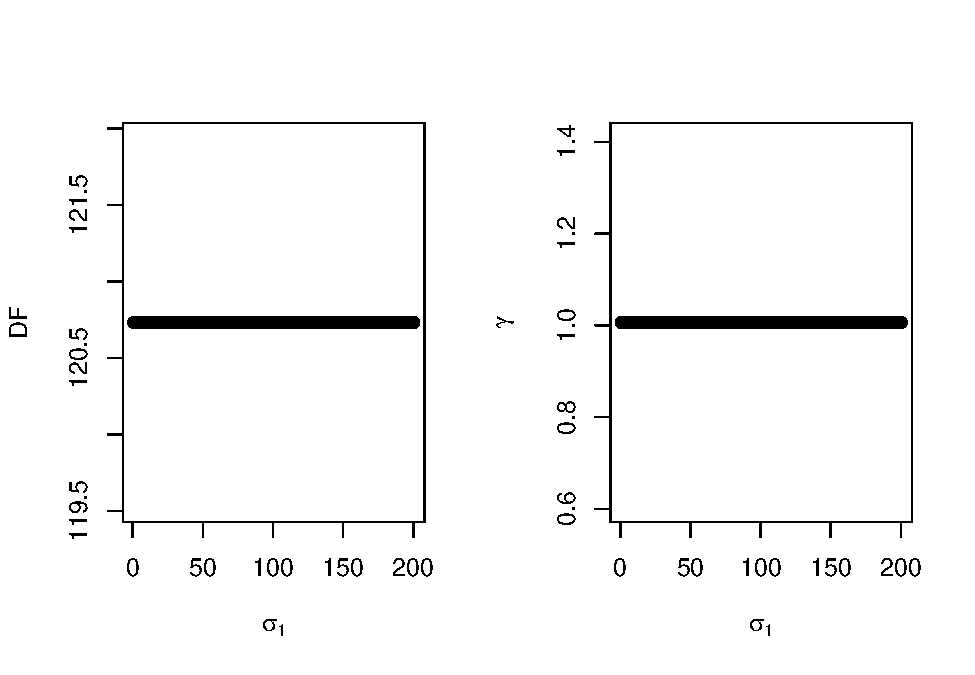
\includegraphics{Theoretical-Bias-of-all-estimators-as-a-function-of-population-parameters_files/figure-latex/biasshiehhetbalvariance2-1.pdf}
\caption{\label{fig:biasshiehhetbalvariance2}Degrees of freedom (DF) and \(\gamma\), when computing the bias of Shieh's \(d_s\), when variances are unequal across groups and sample sizes are equal, as a function of \(\sigma_1\), for a constant \(SD\)-ratio.}
\end{figure}

Note: for a constant \(SD\)-ratio, \(\sigma_1\) and \(\sigma_2\) do not matter (see Figure \ref{fig:biasshiehhetbalvariance2}).

\hypertarget{when-variances-are-unequal-across-populations-with-unequal-sample-sizes-1}{%
\subsubsection{When variances are unequal across populations, with unequal sample sizes}\label{when-variances-are-unequal-across-populations-with-unequal-sample-sizes-1}}

The \textbf{bias} of Shieh's \(d^*_s\) is a function of the population effect size (\(\delta_{Shieh}\)), the sample sizes (\(n_1\) and \(n_2\)), and the interaction between the sample sizes ratio and the \(SD\)-ratio \(\left(\frac{n_1}{n_2}\times\frac{\sigma_1}{\sigma_2} \right)\):

\begin{itemize}
\tightlist
\item
  The larger the population effect size, the more Shieh's \(d_s\) will overestimate \(\delta_{Shieh}\);
\end{itemize}

\begin{figure}
\centering
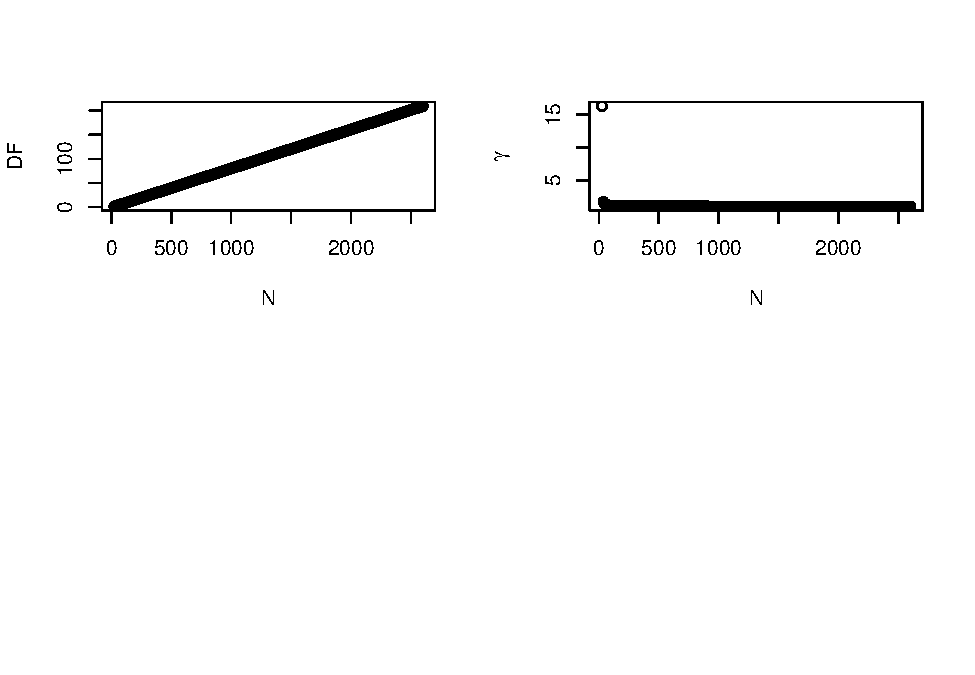
\includegraphics{Theoretical-Bias-of-all-estimators-as-a-function-of-population-parameters_files/figure-latex/biasshiehhetunbalNsize2-1.pdf}
\caption{\label{fig:biasshiehhetunbalNsize2}Degrees of freedom (DF) and \(\gamma\), when computing the bias of Shieh's \(d_s\), when variances and sample sizes are unequal across groups, as a function of the total sample size (\(N\)).}
\end{figure}

\begin{itemize}
\tightlist
\item
  For a constant sample sizes ratio, the larger the sample sizes, the lower the bias (See Figure \ref{fig:biasshiehhetunbalNsize2});
\end{itemize}

\begin{figure}
\centering
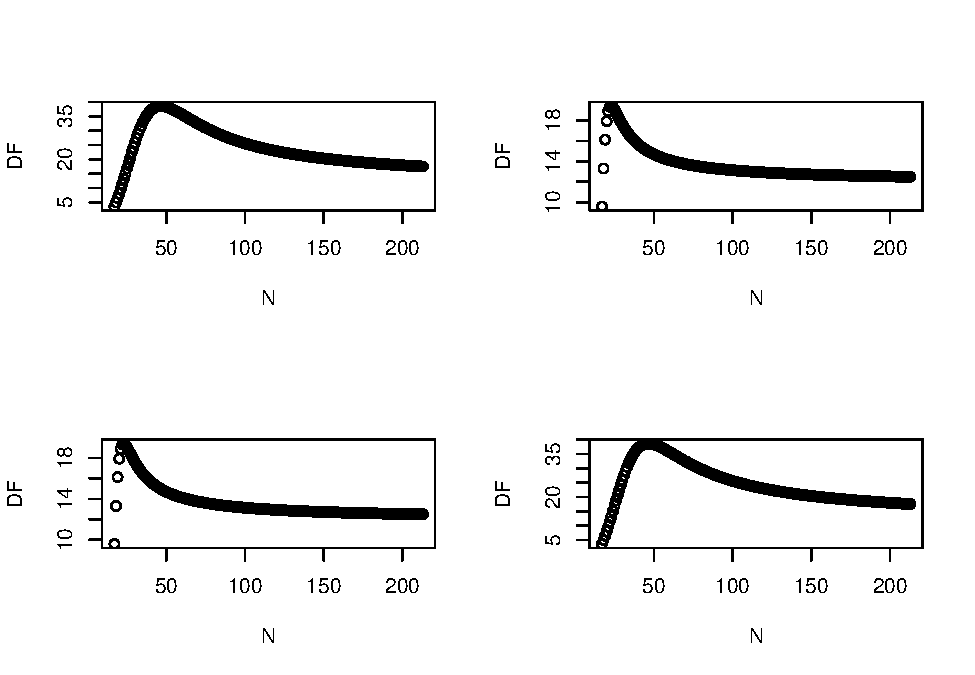
\includegraphics{Theoretical-Bias-of-all-estimators-as-a-function-of-population-parameters_files/figure-latex/biasshiehhetuneqNsize2-1.pdf}
\caption{\label{fig:biasshiehhetuneqNsize2}Degrees of freedom (DF), when computing the bias of Shieh's \(d_s\), when variances and sample sizes are unequal across groups, as a function of the total sample size, when adding subjects only in one group (either in the first group; see top plots; or in the second group; see bottom plots), and \(\sigma_1 > \sigma_2\) (left plots) or \(\sigma_1 < \sigma_2\) (right plots).}
\end{figure}

Note: When variances were equal across populations, adding subjects only in the first group had the same impact on degrees of freedom (and therefore on bias) than adding subjects only in the second group (see Figure \ref{fig:biasshiehhomuneqNsize2}). When variances are unequal across groups, this is not true anymore (see Figure \ref{fig:biasshiehhetuneqNsize2}).

\begin{figure}
\centering
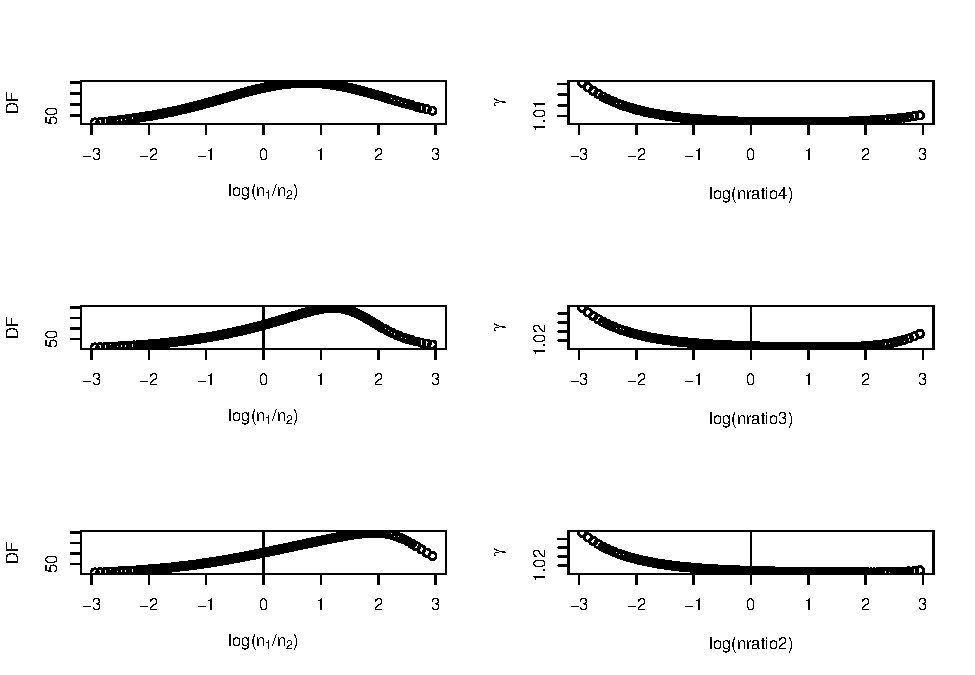
\includegraphics{Theoretical-Bias-of-all-estimators-as-a-function-of-population-parameters_files/figure-latex/biasshiehhetunbaldfandvar-1.pdf}
\caption{\label{fig:biasshiehhetunbaldfandvar}Degrees of freedom (\(DF\)) and \(\gamma\), when computing the bias of Shieh's \(d_s\), when variances and sample sizes are unequal across groups, as a function of the logarithm of the sample sizes ratio (\(log \left( \frac{n_1}{n_2} \right)\)), when \(SD\)-ratio equals 1.46 (first row), 3.39 (second row) or 7 (third row).}
\end{figure}

\begin{itemize}
\tightlist
\item
  The smallest bias always occurs when there is a positive pairing between variances and sample sizes. Moreover, the further the \(SD\)-ratio is from 1, the further from 1 will also be the sample sizes ratio associated with the smallest bias (See Figure \ref{fig:biasshiehhetunbaldfandvar});
\end{itemize}

\begin{figure}
\centering
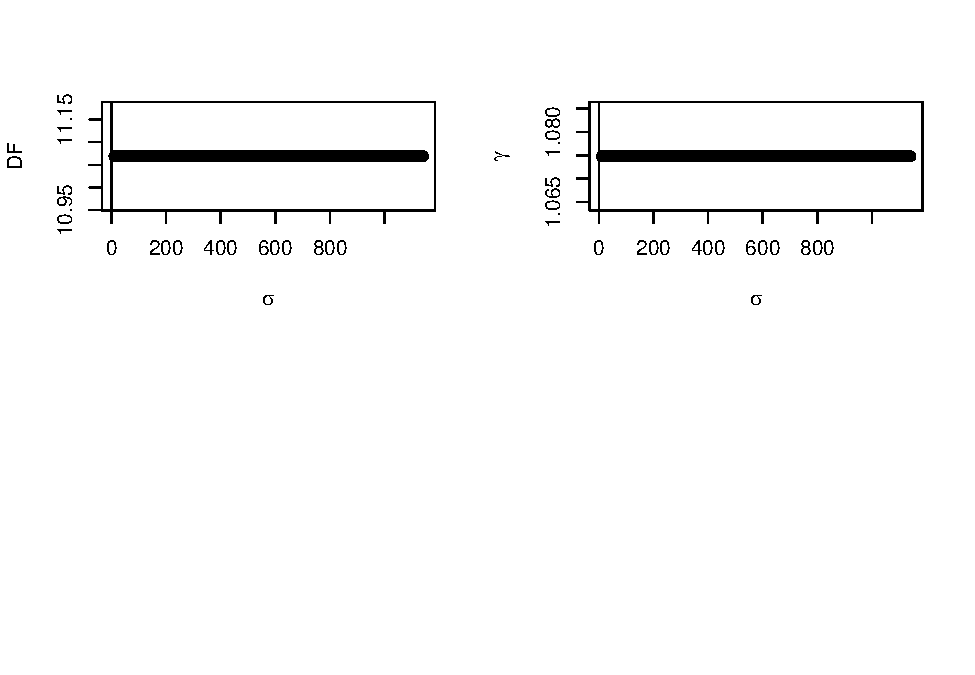
\includegraphics{Theoretical-Bias-of-all-estimators-as-a-function-of-population-parameters_files/figure-latex/biasshiehhetunbalvariance2-1.pdf}
\caption{\label{fig:biasshiehhetunbalvariance2}Degrees of freedom (DF) and \(\gamma\), when computing the bias of Shieh's \(d_s\), when variances and sample sizes are unequal across groups, as a function of \(\sigma_1\) and \(\sigma_2\), for a constant \(SD\)-ratio.}
\end{figure}

Moreover, for a constant \(SD\)-ratio, the variances do not matter (See Figure \ref{fig:biasshiehhetunbalvariance2}).

\hypertarget{in-summary}{%
\subsection{In summary}\label{in-summary}}

The \textbf{bias} of Cohen's \(d_s\) is a function of the population effect size \(\delta_{Cohen}\) and the total sample size (\(N\)):

\begin{itemize}
\tightlist
\item
  When \(\delta_{Cohen}\) is null, the bias is null. In all other configurations, the larger \(\delta_{Cohen}\), the more Cohen's \(d_s\) will overestimate \(\delta_{Cohen}\);\\
\item
  The bias decreases when the total sample size increases (it does not matter whether one adds subjects in only one group or in both).
\end{itemize}

The \textbf{bias} of Glass's \(d_s\) is a function of the population effect size (\(\delta_{Glass}\)) and the size of the control group (\(n_e\)):

\begin{itemize}
\tightlist
\item
  When \(\delta_{Glass}\) is null, the bias is null. In all other configurations, the larger \(\delta_{Glass}\), the more Glass's \(d_s\) will overestimate \(\delta_{Glass}\);\\
\item
  The bias decreases when the size of the control group increases. On the other hand, increasing the size of the experimental group does not impact the bias.
\end{itemize}

The \textbf{bias} of Cohen's \(d^*_s\) is a function of the population effect size (\(\delta^*_{Cohen}\)), the total sample size, and the interaction between the sample sizes ratio and the \(SD\)-ratio \(\left(\frac{n_1}{n_2}\times\frac{\sigma_1}{\sigma_2} \right)\):

\begin{itemize}
\tightlist
\item
  When \(\delta^*_{Cohen}\) is null, the bias is null. In all other configurations, the larger \(\delta^*_{Cohen}\), the more Cohen's \(d^*_s\) will overestimate \(\delta^*_{Cohen}\);\\
\item
  The bias decreases when the total sample size increases (it does not matter whether one adds subjects in only one group or in both);
\item
  The smallest bias always occurs when there is a positive pairing between \(\frac{\sigma_1}{\sigma_1}\) and \(\frac{n_1}{n_1}\). Moreover, the larger the \(SD\)-ratio, the further from 1 is the sample sizes ratio associated with the smallest bias.
\end{itemize}

The \textbf{bias} of Shieh's \(d^*_s\) is a function of the population effect size (\(\delta_{Shieh}\)), the total sample size, and the interaction between the sample sizes ratio and the \(SD\)-ratio \(\left(\frac{n_1}{n_2}\times\frac{\sigma_1}{\sigma_2} \right)\):

\begin{itemize}
\tightlist
\item
  When \(\delta_{Shieh}\) is null, the bias is null. In all other configurations, the larger \(\delta_{Shieh}\), the more Shieh's \(d_s\) will overestimate \(\delta_{Shieh}\);\\
\item
  For a constant sample sizes ratio, the bias decreases when the total sample size increases;\\
\item
  The smallest bias always occurs when there is a positive pairing between \(\frac{\sigma_1}{\sigma_1}\) and \(\frac{n_1}{n_1}\). Moreover, the larger the \(SD\)-ratio, the further from 1 is the sample sizes ratio associated with the smallest bias (for more details, see \enquote{Theoretical Bias, as a function of population parameters}).
\end{itemize}


\end{document}
